\begin{figure}
   \resizebox{\textwidth}{!}{%
        % Created by tikzDevice version 0.12.6 on 2026-06-07 17:41:54
% !TEX encoding = UTF-8 Unicode
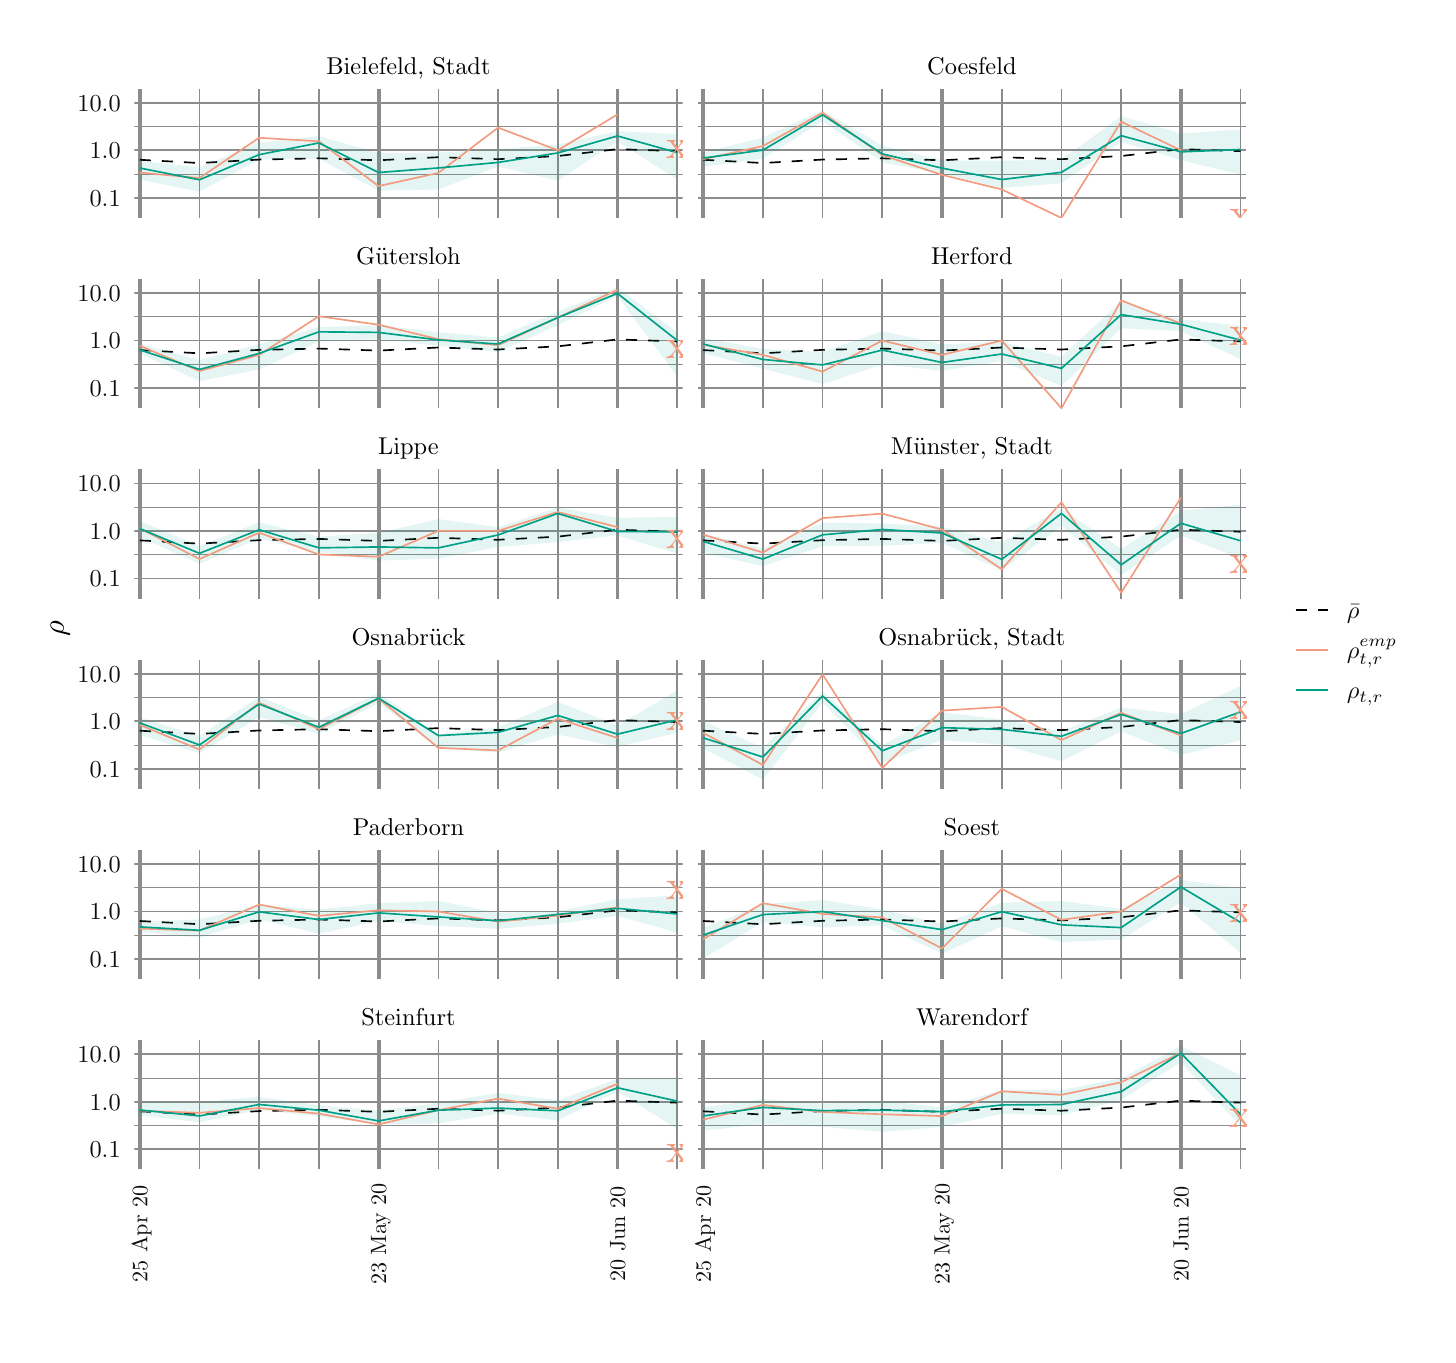
\begin{tikzpicture}[x=1pt,y=1pt]
\definecolor{fillColor}{RGB}{255,255,255}
\path[use as bounding box,fill=fillColor,fill opacity=0.00] (0,0) rectangle (505.89,472.16);
\begin{scope}
\path[clip] ( 38.56,403.40) rectangle (236.65,450.09);
\definecolor{drawColor}{gray}{0.55}

\path[draw=drawColor,line width= 0.3pt,line join=round] ( 38.56,419.27) --
	(236.65,419.27);

\path[draw=drawColor,line width= 0.3pt,line join=round] ( 38.56,436.44) --
	(236.65,436.44);

\path[draw=drawColor,line width= 0.6pt,line join=round] ( 62.08,403.40) --
	( 62.08,450.09);

\path[draw=drawColor,line width= 0.6pt,line join=round] ( 83.65,403.40) --
	( 83.65,450.09);

\path[draw=drawColor,line width= 0.6pt,line join=round] (105.23,403.40) --
	(105.23,450.09);

\path[draw=drawColor,line width= 0.6pt,line join=round] (148.39,403.40) --
	(148.39,450.09);

\path[draw=drawColor,line width= 0.6pt,line join=round] (169.97,403.40) --
	(169.97,450.09);

\path[draw=drawColor,line width= 0.6pt,line join=round] (191.55,403.40) --
	(191.55,450.09);

\path[draw=drawColor,line width= 0.6pt,line join=round] (234.70,403.40) --
	(234.70,450.09);

\path[draw=drawColor,line width= 0.6pt,line join=round] ( 38.56,410.69) --
	(236.65,410.69);

\path[draw=drawColor,line width= 0.6pt,line join=round] ( 38.56,427.85) --
	(236.65,427.85);

\path[draw=drawColor,line width= 0.6pt,line join=round] ( 38.56,445.02) --
	(236.65,445.02);

\path[draw=drawColor,line width= 1.4pt,line join=round] ( 40.50,403.40) --
	( 40.50,450.09);

\path[draw=drawColor,line width= 1.4pt,line join=round] (126.81,403.40) --
	(126.81,450.09);

\path[draw=drawColor,line width= 1.4pt,line join=round] (213.12,403.40) --
	(213.12,450.09);
\definecolor{drawColor}{RGB}{0,0,0}

\path[draw=drawColor,line width= 0.6pt,dash pattern=on 4pt off 4pt ,line join=round] ( 40.50,424.42) --
	( 62.08,423.24) --
	( 83.65,424.49) --
	(105.23,424.95) --
	(126.81,424.23) --
	(148.39,425.35) --
	(169.97,424.63) --
	(191.55,425.77) --
	(213.12,428.27) --
	(234.70,427.54);
\definecolor{fillColor}{RGB}{0,160,135}

\path[fill=fillColor,fill opacity=0.10] ( 40.50,424.07) --
	( 40.50,424.07) --
	( 62.08,421.67) --
	( 62.08,421.67) --
	( 83.65,430.66) --
	( 83.65,430.66) --
	(105.23,432.92) --
	(105.23,432.92) --
	(126.81,426.88) --
	(126.81,426.88) --
	(148.39,426.99) --
	(148.39,426.99) --
	(169.97,428.21) --
	(169.97,428.21) --
	(191.55,429.94) --
	(191.55,429.94) --
	(213.12,434.74) --
	(213.12,434.74) --
	(234.70,433.74) --
	(234.70,433.74) --
	(234.70,417.31) --
	(234.70,417.31) --
	(213.12,431.01) --
	(213.12,431.01) --
	(191.55,416.91) --
	(191.55,416.91) --
	(169.97,421.97) --
	(169.97,421.97) --
	(148.39,413.68) --
	(148.39,413.68) --
	(126.81,413.28) --
	(126.81,413.28) --
	(105.23,424.82) --
	(105.23,424.82) --
	( 83.65,424.47) --
	( 83.65,424.47) --
	( 62.08,412.88) --
	( 62.08,412.88) --
	( 40.50,417.23) --
	( 40.50,417.23) --
	cycle;

\path[] ( 40.50,424.07) --
	( 40.50,424.07) --
	( 62.08,421.67) --
	( 62.08,421.67) --
	( 83.65,430.66) --
	( 83.65,430.66) --
	(105.23,432.92) --
	(105.23,432.92) --
	(126.81,426.88) --
	(126.81,426.88) --
	(148.39,426.99) --
	(148.39,426.99) --
	(169.97,428.21) --
	(169.97,428.21) --
	(191.55,429.94) --
	(191.55,429.94) --
	(213.12,434.74) --
	(213.12,434.74) --
	(234.70,433.74) --
	(234.70,433.74);

\path[] (234.70,417.31) --
	(234.70,417.31) --
	(213.12,431.01) --
	(213.12,431.01) --
	(191.55,416.91) --
	(191.55,416.91) --
	(169.97,421.97) --
	(169.97,421.97) --
	(148.39,413.68) --
	(148.39,413.68) --
	(126.81,413.28) --
	(126.81,413.28) --
	(105.23,424.82) --
	(105.23,424.82) --
	( 83.65,424.47) --
	( 83.65,424.47) --
	( 62.08,412.88) --
	( 62.08,412.88) --
	( 40.50,417.23) --
	( 40.50,417.23);
\definecolor{drawColor}{RGB}{243,155,127}

\path[draw=drawColor,line width= 0.6pt,line join=round] ( 40.50,419.77) --
	( 62.08,417.84) --
	( 83.65,432.37) --
	(105.23,431.10) --
	(126.81,414.92) --
	(148.39,419.66) --
	(169.97,436.04) --
	(191.55,427.85) --
	(213.12,440.78);
\definecolor{drawColor}{RGB}{0,160,135}

\path[draw=drawColor,line width= 0.6pt,line join=round] ( 40.50,421.43) --
	( 62.08,417.19) --
	( 83.65,426.27) --
	(105.23,430.51) --
	(126.81,419.82) --
	(148.39,421.46) --
	(169.97,423.46) --
	(191.55,426.88) --
	(213.12,433.02) --
	(234.70,427.02);
\definecolor{drawColor}{RGB}{243,155,127}

\node[text=drawColor,anchor=base,inner sep=0pt, outer sep=0pt, scale=  1.52] at (234.70,425.01) {x};
\end{scope}
\begin{scope}
\path[clip] ( 38.56,334.63) rectangle (236.65,381.33);
\definecolor{drawColor}{gray}{0.55}

\path[draw=drawColor,line width= 0.3pt,line join=round] ( 38.56,350.51) --
	(236.65,350.51);

\path[draw=drawColor,line width= 0.3pt,line join=round] ( 38.56,367.67) --
	(236.65,367.67);

\path[draw=drawColor,line width= 0.6pt,line join=round] ( 62.08,334.63) --
	( 62.08,381.33);

\path[draw=drawColor,line width= 0.6pt,line join=round] ( 83.65,334.63) --
	( 83.65,381.33);

\path[draw=drawColor,line width= 0.6pt,line join=round] (105.23,334.63) --
	(105.23,381.33);

\path[draw=drawColor,line width= 0.6pt,line join=round] (148.39,334.63) --
	(148.39,381.33);

\path[draw=drawColor,line width= 0.6pt,line join=round] (169.97,334.63) --
	(169.97,381.33);

\path[draw=drawColor,line width= 0.6pt,line join=round] (191.55,334.63) --
	(191.55,381.33);

\path[draw=drawColor,line width= 0.6pt,line join=round] (234.70,334.63) --
	(234.70,381.33);

\path[draw=drawColor,line width= 0.6pt,line join=round] ( 38.56,341.92) --
	(236.65,341.92);

\path[draw=drawColor,line width= 0.6pt,line join=round] ( 38.56,359.09) --
	(236.65,359.09);

\path[draw=drawColor,line width= 0.6pt,line join=round] ( 38.56,376.25) --
	(236.65,376.25);

\path[draw=drawColor,line width= 1.4pt,line join=round] ( 40.50,334.63) --
	( 40.50,381.33);

\path[draw=drawColor,line width= 1.4pt,line join=round] (126.81,334.63) --
	(126.81,381.33);

\path[draw=drawColor,line width= 1.4pt,line join=round] (213.12,334.63) --
	(213.12,381.33);
\definecolor{drawColor}{RGB}{0,0,0}

\path[draw=drawColor,line width= 0.6pt,dash pattern=on 4pt off 4pt ,line join=round] ( 40.50,355.65) --
	( 62.08,354.48) --
	( 83.65,355.73) --
	(105.23,356.19) --
	(126.81,355.47) --
	(148.39,356.58) --
	(169.97,355.86) --
	(191.55,357.00) --
	(213.12,359.50) --
	(234.70,358.77);
\definecolor{fillColor}{RGB}{0,160,135}

\path[fill=fillColor,fill opacity=0.10] ( 40.50,357.96) --
	( 40.50,357.96) --
	( 62.08,352.05) --
	( 62.08,352.05) --
	( 83.65,357.74) --
	( 83.65,357.74) --
	(105.23,363.95) --
	(105.23,363.95) --
	(126.81,364.63) --
	(126.81,364.63) --
	(148.39,362.15) --
	(148.39,362.15) --
	(169.97,360.15) --
	(169.97,360.15) --
	(191.55,369.56) --
	(191.55,369.56) --
	(213.12,378.33) --
	(213.12,378.33) --
	(234.70,361.96) --
	(234.70,361.96) --
	(234.70,346.12) --
	(234.70,346.12) --
	(213.12,375.24) --
	(213.12,375.24) --
	(191.55,364.65) --
	(191.55,364.65) --
	(169.97,354.97) --
	(169.97,354.97) --
	(148.39,357.20) --
	(148.39,357.20) --
	(126.81,359.60) --
	(126.81,359.60) --
	(105.23,358.78) --
	(105.23,358.78) --
	( 83.65,348.63) --
	( 83.65,348.63) --
	( 62.08,344.43) --
	( 62.08,344.43) --
	( 40.50,354.46) --
	( 40.50,354.46) --
	cycle;

\path[] ( 40.50,357.96) --
	( 40.50,357.96) --
	( 62.08,352.05) --
	( 62.08,352.05) --
	( 83.65,357.74) --
	( 83.65,357.74) --
	(105.23,363.95) --
	(105.23,363.95) --
	(126.81,364.63) --
	(126.81,364.63) --
	(148.39,362.15) --
	(148.39,362.15) --
	(169.97,360.15) --
	(169.97,360.15) --
	(191.55,369.56) --
	(191.55,369.56) --
	(213.12,378.33) --
	(213.12,378.33) --
	(234.70,361.96) --
	(234.70,361.96);

\path[] (234.70,346.12) --
	(234.70,346.12) --
	(213.12,375.24) --
	(213.12,375.24) --
	(191.55,364.65) --
	(191.55,364.65) --
	(169.97,354.97) --
	(169.97,354.97) --
	(148.39,357.20) --
	(148.39,357.20) --
	(126.81,359.60) --
	(126.81,359.60) --
	(105.23,358.78) --
	(105.23,358.78) --
	( 83.65,348.63) --
	( 83.65,348.63) --
	( 62.08,344.43) --
	( 62.08,344.43) --
	( 40.50,354.46) --
	( 40.50,354.46);
\definecolor{drawColor}{RGB}{243,155,127}

\path[draw=drawColor,line width= 0.6pt,line join=round] ( 40.50,357.21) --
	( 62.08,348.09) --
	( 83.65,353.92) --
	(105.23,367.87) --
	(126.81,364.81) --
	(148.39,359.60) --
	(169.97,357.42) --
	(191.55,367.38) --
	(213.12,377.44);
\definecolor{drawColor}{RGB}{0,160,135}

\path[draw=drawColor,line width= 0.6pt,line join=round] ( 40.50,355.73) --
	( 62.08,348.65) --
	( 83.65,354.45) --
	(105.23,362.25) --
	(126.81,362.04) --
	(148.39,359.31) --
	(169.97,357.85) --
	(191.55,367.39) --
	(213.12,376.12) --
	(234.70,359.12);
\definecolor{drawColor}{RGB}{243,155,127}

\node[text=drawColor,anchor=base,inner sep=0pt, outer sep=0pt, scale=  1.52] at (234.70,352.62) {x};
\end{scope}
\begin{scope}
\path[clip] ( 38.56,265.87) rectangle (236.65,312.56);
\definecolor{drawColor}{gray}{0.55}

\path[draw=drawColor,line width= 0.3pt,line join=round] ( 38.56,281.74) --
	(236.65,281.74);

\path[draw=drawColor,line width= 0.3pt,line join=round] ( 38.56,298.90) --
	(236.65,298.90);

\path[draw=drawColor,line width= 0.6pt,line join=round] ( 62.08,265.87) --
	( 62.08,312.56);

\path[draw=drawColor,line width= 0.6pt,line join=round] ( 83.65,265.87) --
	( 83.65,312.56);

\path[draw=drawColor,line width= 0.6pt,line join=round] (105.23,265.87) --
	(105.23,312.56);

\path[draw=drawColor,line width= 0.6pt,line join=round] (148.39,265.87) --
	(148.39,312.56);

\path[draw=drawColor,line width= 0.6pt,line join=round] (169.97,265.87) --
	(169.97,312.56);

\path[draw=drawColor,line width= 0.6pt,line join=round] (191.55,265.87) --
	(191.55,312.56);

\path[draw=drawColor,line width= 0.6pt,line join=round] (234.70,265.87) --
	(234.70,312.56);

\path[draw=drawColor,line width= 0.6pt,line join=round] ( 38.56,273.16) --
	(236.65,273.16);

\path[draw=drawColor,line width= 0.6pt,line join=round] ( 38.56,290.32) --
	(236.65,290.32);

\path[draw=drawColor,line width= 0.6pt,line join=round] ( 38.56,307.49) --
	(236.65,307.49);

\path[draw=drawColor,line width= 1.4pt,line join=round] ( 40.50,265.87) --
	( 40.50,312.56);

\path[draw=drawColor,line width= 1.4pt,line join=round] (126.81,265.87) --
	(126.81,312.56);

\path[draw=drawColor,line width= 1.4pt,line join=round] (213.12,265.87) --
	(213.12,312.56);
\definecolor{drawColor}{RGB}{0,0,0}

\path[draw=drawColor,line width= 0.6pt,dash pattern=on 4pt off 4pt ,line join=round] ( 40.50,286.89) --
	( 62.08,285.71) --
	( 83.65,286.96) --
	(105.23,287.42) --
	(126.81,286.70) --
	(148.39,287.82) --
	(169.97,287.10) --
	(191.55,288.24) --
	(213.12,290.74) --
	(234.70,290.01);
\definecolor{fillColor}{RGB}{0,160,135}

\path[fill=fillColor,fill opacity=0.10] ( 40.50,293.88) --
	( 40.50,293.88) --
	( 62.08,284.91) --
	( 62.08,284.91) --
	( 83.65,293.38) --
	( 83.65,293.38) --
	(105.23,288.26) --
	(105.23,288.26) --
	(126.81,289.59) --
	(126.81,289.59) --
	(148.39,294.59) --
	(148.39,294.59) --
	(169.97,291.65) --
	(169.97,291.65) --
	(191.55,298.78) --
	(191.55,298.78) --
	(213.12,295.06) --
	(213.12,295.06) --
	(234.70,295.36) --
	(234.70,295.36) --
	(234.70,282.13) --
	(234.70,282.13) --
	(213.12,288.73) --
	(213.12,288.73) --
	(191.55,286.25) --
	(191.55,286.25) --
	(169.97,284.49) --
	(169.97,284.49) --
	(148.39,280.33) --
	(148.39,280.33) --
	(126.81,279.58) --
	(126.81,279.58) --
	(105.23,282.64) --
	(105.23,282.64) --
	( 83.65,287.57) --
	( 83.65,287.57) --
	( 62.08,278.40) --
	( 62.08,278.40) --
	( 40.50,288.13) --
	( 40.50,288.13) --
	cycle;

\path[] ( 40.50,293.88) --
	( 40.50,293.88) --
	( 62.08,284.91) --
	( 62.08,284.91) --
	( 83.65,293.38) --
	( 83.65,293.38) --
	(105.23,288.26) --
	(105.23,288.26) --
	(126.81,289.59) --
	(126.81,289.59) --
	(148.39,294.59) --
	(148.39,294.59) --
	(169.97,291.65) --
	(169.97,291.65) --
	(191.55,298.78) --
	(191.55,298.78) --
	(213.12,295.06) --
	(213.12,295.06) --
	(234.70,295.36) --
	(234.70,295.36);

\path[] (234.70,282.13) --
	(234.70,282.13) --
	(213.12,288.73) --
	(213.12,288.73) --
	(191.55,286.25) --
	(191.55,286.25) --
	(169.97,284.49) --
	(169.97,284.49) --
	(148.39,280.33) --
	(148.39,280.33) --
	(126.81,279.58) --
	(126.81,279.58) --
	(105.23,282.64) --
	(105.23,282.64) --
	( 83.65,287.57) --
	( 83.65,287.57) --
	( 62.08,278.40) --
	( 62.08,278.40) --
	( 40.50,288.13) --
	( 40.50,288.13);
\definecolor{drawColor}{RGB}{243,155,127}

\path[draw=drawColor,line width= 0.6pt,line join=round] ( 40.50,291.25) --
	( 62.08,280.15) --
	( 83.65,289.67) --
	(105.23,281.79) --
	(126.81,280.98) --
	(148.39,290.32) --
	(169.97,290.32) --
	(191.55,297.15) --
	(213.12,291.68);
\definecolor{drawColor}{RGB}{0,160,135}

\path[draw=drawColor,line width= 0.6pt,line join=round] ( 40.50,291.14) --
	( 62.08,282.21) --
	( 83.65,290.73) --
	(105.23,284.19) --
	(126.81,284.52) --
	(148.39,284.17) --
	(169.97,288.84) --
	(191.55,296.62) --
	(213.12,290.11) --
	(234.70,289.95);
\definecolor{drawColor}{RGB}{243,155,127}

\node[text=drawColor,anchor=base,inner sep=0pt, outer sep=0pt, scale=  1.52] at (234.70,284.03) {x};
\end{scope}
\begin{scope}
\path[clip] ( 38.56,197.10) rectangle (236.65,243.80);
\definecolor{drawColor}{gray}{0.55}

\path[draw=drawColor,line width= 0.3pt,line join=round] ( 38.56,212.97) --
	(236.65,212.97);

\path[draw=drawColor,line width= 0.3pt,line join=round] ( 38.56,230.14) --
	(236.65,230.14);

\path[draw=drawColor,line width= 0.6pt,line join=round] ( 62.08,197.10) --
	( 62.08,243.80);

\path[draw=drawColor,line width= 0.6pt,line join=round] ( 83.65,197.10) --
	( 83.65,243.80);

\path[draw=drawColor,line width= 0.6pt,line join=round] (105.23,197.10) --
	(105.23,243.80);

\path[draw=drawColor,line width= 0.6pt,line join=round] (148.39,197.10) --
	(148.39,243.80);

\path[draw=drawColor,line width= 0.6pt,line join=round] (169.97,197.10) --
	(169.97,243.80);

\path[draw=drawColor,line width= 0.6pt,line join=round] (191.55,197.10) --
	(191.55,243.80);

\path[draw=drawColor,line width= 0.6pt,line join=round] (234.70,197.10) --
	(234.70,243.80);

\path[draw=drawColor,line width= 0.6pt,line join=round] ( 38.56,204.39) --
	(236.65,204.39);

\path[draw=drawColor,line width= 0.6pt,line join=round] ( 38.56,221.56) --
	(236.65,221.56);

\path[draw=drawColor,line width= 0.6pt,line join=round] ( 38.56,238.72) --
	(236.65,238.72);

\path[draw=drawColor,line width= 1.4pt,line join=round] ( 40.50,197.10) --
	( 40.50,243.80);

\path[draw=drawColor,line width= 1.4pt,line join=round] (126.81,197.10) --
	(126.81,243.80);

\path[draw=drawColor,line width= 1.4pt,line join=round] (213.12,197.10) --
	(213.12,243.80);
\definecolor{drawColor}{RGB}{0,0,0}

\path[draw=drawColor,line width= 0.6pt,dash pattern=on 4pt off 4pt ,line join=round] ( 40.50,218.12) --
	( 62.08,216.95) --
	( 83.65,218.20) --
	(105.23,218.66) --
	(126.81,217.94) --
	(148.39,219.05) --
	(169.97,218.33) --
	(191.55,219.47) --
	(213.12,221.97) --
	(234.70,221.24);
\definecolor{fillColor}{RGB}{0,160,135}

\path[fill=fillColor,fill opacity=0.10] ( 40.50,222.91) --
	( 40.50,222.91) --
	( 62.08,216.27) --
	( 62.08,216.27) --
	( 83.65,230.35) --
	( 83.65,230.35) --
	(105.23,221.84) --
	(105.23,221.84) --
	(126.81,231.68) --
	(126.81,231.68) --
	(148.39,216.76) --
	(148.39,216.76) --
	(169.97,219.34) --
	(169.97,219.34) --
	(191.55,228.61) --
	(191.55,228.61) --
	(213.12,219.96) --
	(213.12,219.96) --
	(234.70,232.68) --
	(234.70,232.68) --
	(234.70,217.35) --
	(234.70,217.35) --
	(213.12,212.28) --
	(213.12,212.28) --
	(191.55,216.72) --
	(191.55,216.72) --
	(169.97,210.19) --
	(169.97,210.19) --
	(148.39,211.80) --
	(148.39,211.80) --
	(126.81,228.11) --
	(126.81,228.11) --
	(105.23,217.02) --
	(105.23,217.02) --
	( 83.65,223.01) --
	( 83.65,223.01) --
	( 62.08,209.96) --
	( 62.08,209.96) --
	( 40.50,216.57) --
	( 40.50,216.57) --
	cycle;

\path[] ( 40.50,222.91) --
	( 40.50,222.91) --
	( 62.08,216.27) --
	( 62.08,216.27) --
	( 83.65,230.35) --
	( 83.65,230.35) --
	(105.23,221.84) --
	(105.23,221.84) --
	(126.81,231.68) --
	(126.81,231.68) --
	(148.39,216.76) --
	(148.39,216.76) --
	(169.97,219.34) --
	(169.97,219.34) --
	(191.55,228.61) --
	(191.55,228.61) --
	(213.12,219.96) --
	(213.12,219.96) --
	(234.70,232.68) --
	(234.70,232.68);

\path[] (234.70,217.35) --
	(234.70,217.35) --
	(213.12,212.28) --
	(213.12,212.28) --
	(191.55,216.72) --
	(191.55,216.72) --
	(169.97,210.19) --
	(169.97,210.19) --
	(148.39,211.80) --
	(148.39,211.80) --
	(126.81,228.11) --
	(126.81,228.11) --
	(105.23,217.02) --
	(105.23,217.02) --
	( 83.65,223.01) --
	( 83.65,223.01) --
	( 62.08,209.96) --
	( 62.08,209.96) --
	( 40.50,216.57) --
	( 40.50,216.57);
\definecolor{drawColor}{RGB}{243,155,127}

\path[draw=drawColor,line width= 0.6pt,line join=round] ( 40.50,220.20) --
	( 62.08,211.30) --
	( 83.65,228.26) --
	(105.23,218.66) --
	(126.81,229.75) --
	(148.39,211.93) --
	(169.97,210.99) --
	(191.55,222.44) --
	(213.12,215.51);
\definecolor{drawColor}{RGB}{0,160,135}

\path[draw=drawColor,line width= 0.6pt,line join=round] ( 40.50,220.94) --
	( 62.08,212.98) --
	( 83.65,227.75) --
	(105.23,219.36) --
	(126.81,229.87) --
	(148.39,216.36) --
	(169.97,217.52) --
	(191.55,223.63) --
	(213.12,216.86) --
	(234.70,222.04);
\definecolor{drawColor}{RGB}{243,155,127}

\node[text=drawColor,anchor=base,inner sep=0pt, outer sep=0pt, scale=  1.52] at (234.70,218.29) {x};
\end{scope}
\begin{scope}
\path[clip] ( 38.56,128.34) rectangle (236.65,175.03);
\definecolor{drawColor}{gray}{0.55}

\path[draw=drawColor,line width= 0.3pt,line join=round] ( 38.56,144.21) --
	(236.65,144.21);

\path[draw=drawColor,line width= 0.3pt,line join=round] ( 38.56,161.37) --
	(236.65,161.37);

\path[draw=drawColor,line width= 0.6pt,line join=round] ( 62.08,128.34) --
	( 62.08,175.03);

\path[draw=drawColor,line width= 0.6pt,line join=round] ( 83.65,128.34) --
	( 83.65,175.03);

\path[draw=drawColor,line width= 0.6pt,line join=round] (105.23,128.34) --
	(105.23,175.03);

\path[draw=drawColor,line width= 0.6pt,line join=round] (148.39,128.34) --
	(148.39,175.03);

\path[draw=drawColor,line width= 0.6pt,line join=round] (169.97,128.34) --
	(169.97,175.03);

\path[draw=drawColor,line width= 0.6pt,line join=round] (191.55,128.34) --
	(191.55,175.03);

\path[draw=drawColor,line width= 0.6pt,line join=round] (234.70,128.34) --
	(234.70,175.03);

\path[draw=drawColor,line width= 0.6pt,line join=round] ( 38.56,135.63) --
	(236.65,135.63);

\path[draw=drawColor,line width= 0.6pt,line join=round] ( 38.56,152.79) --
	(236.65,152.79);

\path[draw=drawColor,line width= 0.6pt,line join=round] ( 38.56,169.96) --
	(236.65,169.96);

\path[draw=drawColor,line width= 1.4pt,line join=round] ( 40.50,128.34) --
	( 40.50,175.03);

\path[draw=drawColor,line width= 1.4pt,line join=round] (126.81,128.34) --
	(126.81,175.03);

\path[draw=drawColor,line width= 1.4pt,line join=round] (213.12,128.34) --
	(213.12,175.03);
\definecolor{drawColor}{RGB}{0,0,0}

\path[draw=drawColor,line width= 0.6pt,dash pattern=on 4pt off 4pt ,line join=round] ( 40.50,149.36) --
	( 62.08,148.18) --
	( 83.65,149.43) --
	(105.23,149.89) --
	(126.81,149.17) --
	(148.39,150.29) --
	(169.97,149.57) --
	(191.55,150.70) --
	(213.12,153.20) --
	(234.70,152.48);
\definecolor{fillColor}{RGB}{0,160,135}

\path[fill=fillColor,fill opacity=0.10] ( 40.50,149.02) --
	( 40.50,149.02) --
	( 62.08,149.91) --
	( 62.08,149.91) --
	( 83.65,155.18) --
	( 83.65,155.18) --
	(105.23,153.49) --
	(105.23,153.49) --
	(126.81,155.77) --
	(126.81,155.77) --
	(148.39,156.62) --
	(148.39,156.62) --
	(169.97,152.27) --
	(169.97,152.27) --
	(191.55,152.88) --
	(191.55,152.88) --
	(213.12,157.26) --
	(213.12,157.26) --
	(234.70,158.65) --
	(234.70,158.65) --
	(234.70,145.18) --
	(234.70,145.18) --
	(213.12,151.19) --
	(213.12,151.19) --
	(191.55,148.37) --
	(191.55,148.37) --
	(169.97,146.53) --
	(169.97,146.53) --
	(148.39,147.59) --
	(148.39,147.59) --
	(126.81,149.33) --
	(126.81,149.33) --
	(105.23,144.80) --
	(105.23,144.80) --
	( 83.65,149.90) --
	( 83.65,149.90) --
	( 62.08,143.40) --
	( 62.08,143.40) --
	( 40.50,145.29) --
	( 40.50,145.29) --
	cycle;

\path[] ( 40.50,149.02) --
	( 40.50,149.02) --
	( 62.08,149.91) --
	( 62.08,149.91) --
	( 83.65,155.18) --
	( 83.65,155.18) --
	(105.23,153.49) --
	(105.23,153.49) --
	(126.81,155.77) --
	(126.81,155.77) --
	(148.39,156.62) --
	(148.39,156.62) --
	(169.97,152.27) --
	(169.97,152.27) --
	(191.55,152.88) --
	(191.55,152.88) --
	(213.12,157.26) --
	(213.12,157.26) --
	(234.70,158.65) --
	(234.70,158.65);

\path[] (234.70,145.18) --
	(234.70,145.18) --
	(213.12,151.19) --
	(213.12,151.19) --
	(191.55,148.37) --
	(191.55,148.37) --
	(169.97,146.53) --
	(169.97,146.53) --
	(148.39,147.59) --
	(148.39,147.59) --
	(126.81,149.33) --
	(126.81,149.33) --
	(105.23,144.80) --
	(105.23,144.80) --
	( 83.65,149.90) --
	( 83.65,149.90) --
	( 62.08,143.40) --
	( 62.08,143.40) --
	( 40.50,145.29) --
	( 40.50,145.29);
\definecolor{drawColor}{RGB}{243,155,127}

\path[draw=drawColor,line width= 0.6pt,line join=round] ( 40.50,146.62) --
	( 62.08,145.86) --
	( 83.65,155.30) --
	(105.23,151.22) --
	(126.81,153.22) --
	(148.39,152.79) --
	(169.97,149.12) --
	(191.55,151.30) --
	(213.12,154.29);
\definecolor{drawColor}{RGB}{0,160,135}

\path[draw=drawColor,line width= 0.6pt,line join=round] ( 40.50,147.23) --
	( 62.08,145.99) --
	( 83.65,152.66) --
	(105.23,149.89) --
	(126.81,152.28) --
	(148.39,150.83) --
	(169.97,149.44) --
	(191.55,151.74) --
	(213.12,153.92) --
	(234.70,151.90);
\definecolor{drawColor}{RGB}{243,155,127}

\node[text=drawColor,anchor=base,inner sep=0pt, outer sep=0pt, scale=  1.52] at (234.70,157.01) {x};
\end{scope}
\begin{scope}
\path[clip] ( 38.56, 59.57) rectangle (236.65,106.27);
\definecolor{drawColor}{gray}{0.55}

\path[draw=drawColor,line width= 0.3pt,line join=round] ( 38.56, 75.44) --
	(236.65, 75.44);

\path[draw=drawColor,line width= 0.3pt,line join=round] ( 38.56, 92.61) --
	(236.65, 92.61);

\path[draw=drawColor,line width= 0.6pt,line join=round] ( 62.08, 59.57) --
	( 62.08,106.27);

\path[draw=drawColor,line width= 0.6pt,line join=round] ( 83.65, 59.57) --
	( 83.65,106.27);

\path[draw=drawColor,line width= 0.6pt,line join=round] (105.23, 59.57) --
	(105.23,106.27);

\path[draw=drawColor,line width= 0.6pt,line join=round] (148.39, 59.57) --
	(148.39,106.27);

\path[draw=drawColor,line width= 0.6pt,line join=round] (169.97, 59.57) --
	(169.97,106.27);

\path[draw=drawColor,line width= 0.6pt,line join=round] (191.55, 59.57) --
	(191.55,106.27);

\path[draw=drawColor,line width= 0.6pt,line join=round] (234.70, 59.57) --
	(234.70,106.27);

\path[draw=drawColor,line width= 0.6pt,line join=round] ( 38.56, 66.86) --
	(236.65, 66.86);

\path[draw=drawColor,line width= 0.6pt,line join=round] ( 38.56, 84.03) --
	(236.65, 84.03);

\path[draw=drawColor,line width= 0.6pt,line join=round] ( 38.56,101.19) --
	(236.65,101.19);

\path[draw=drawColor,line width= 1.4pt,line join=round] ( 40.50, 59.57) --
	( 40.50,106.27);

\path[draw=drawColor,line width= 1.4pt,line join=round] (126.81, 59.57) --
	(126.81,106.27);

\path[draw=drawColor,line width= 1.4pt,line join=round] (213.12, 59.57) --
	(213.12,106.27);
\definecolor{drawColor}{RGB}{0,0,0}

\path[draw=drawColor,line width= 0.6pt,dash pattern=on 4pt off 4pt ,line join=round] ( 40.50, 80.59) --
	( 62.08, 79.41) --
	( 83.65, 80.67) --
	(105.23, 81.13) --
	(126.81, 80.40) --
	(148.39, 81.52) --
	(169.97, 80.80) --
	(191.55, 81.94) --
	(213.12, 84.44) --
	(234.70, 83.71);
\definecolor{fillColor}{RGB}{0,160,135}

\path[fill=fillColor,fill opacity=0.10] ( 40.50, 84.12) --
	( 40.50, 84.12) --
	( 62.08, 83.84) --
	( 62.08, 83.84) --
	( 83.65, 85.81) --
	( 83.65, 85.81) --
	(105.23, 82.79) --
	(105.23, 82.79) --
	(126.81, 80.93) --
	(126.81, 80.93) --
	(148.39, 83.61) --
	(148.39, 83.61) --
	(169.97, 87.24) --
	(169.97, 87.24) --
	(191.55, 84.58) --
	(191.55, 84.58) --
	(213.12, 92.35) --
	(213.12, 92.35) --
	(234.70, 92.61) --
	(234.70, 92.61) --
	(234.70, 74.24) --
	(234.70, 74.24) --
	(213.12, 87.73) --
	(213.12, 87.73) --
	(191.55, 77.29) --
	(191.55, 77.29) --
	(169.97, 79.81) --
	(169.97, 79.81) --
	(148.39, 76.20) --
	(148.39, 76.20) --
	(126.81, 75.94) --
	(126.81, 75.94) --
	(105.23, 78.69) --
	(105.23, 78.69) --
	( 83.65, 81.12) --
	( 83.65, 81.12) --
	( 62.08, 76.69) --
	( 62.08, 76.69) --
	( 40.50, 79.13) --
	( 40.50, 79.13) --
	cycle;

\path[] ( 40.50, 84.12) --
	( 40.50, 84.12) --
	( 62.08, 83.84) --
	( 62.08, 83.84) --
	( 83.65, 85.81) --
	( 83.65, 85.81) --
	(105.23, 82.79) --
	(105.23, 82.79) --
	(126.81, 80.93) --
	(126.81, 80.93) --
	(148.39, 83.61) --
	(148.39, 83.61) --
	(169.97, 87.24) --
	(169.97, 87.24) --
	(191.55, 84.58) --
	(191.55, 84.58) --
	(213.12, 92.35) --
	(213.12, 92.35) --
	(234.70, 92.61) --
	(234.70, 92.61);

\path[] (234.70, 74.24) --
	(234.70, 74.24) --
	(213.12, 87.73) --
	(213.12, 87.73) --
	(191.55, 77.29) --
	(191.55, 77.29) --
	(169.97, 79.81) --
	(169.97, 79.81) --
	(148.39, 76.20) --
	(148.39, 76.20) --
	(126.81, 75.94) --
	(126.81, 75.94) --
	(105.23, 78.69) --
	(105.23, 78.69) --
	( 83.65, 81.12) --
	( 83.65, 81.12) --
	( 62.08, 76.69) --
	( 62.08, 76.69) --
	( 40.50, 79.13) --
	( 40.50, 79.13);
\definecolor{drawColor}{RGB}{243,155,127}

\path[draw=drawColor,line width= 0.6pt,line join=round] ( 40.50, 80.81) --
	( 62.08, 80.04) --
	( 83.65, 81.77) --
	(105.23, 79.74) --
	(126.81, 75.84) --
	(148.39, 81.00) --
	(169.97, 85.18) --
	(191.55, 81.52) --
	(213.12, 90.55);
\definecolor{drawColor}{RGB}{0,160,135}

\path[draw=drawColor,line width= 0.6pt,line join=round] ( 40.50, 81.07) --
	( 62.08, 78.91) --
	( 83.65, 83.05) --
	(105.23, 80.98) --
	(126.81, 77.11) --
	(148.39, 80.99) --
	(169.97, 81.75) --
	(191.55, 80.76) --
	(213.12, 89.10) --
	(234.70, 84.27);
\definecolor{drawColor}{RGB}{243,155,127}

\node[text=drawColor,anchor=base,inner sep=0pt, outer sep=0pt, scale=  1.52] at (234.70, 62.24) {x};
\end{scope}
\begin{scope}
\path[clip] (242.15,403.40) rectangle (440.24,450.09);
\definecolor{drawColor}{gray}{0.55}

\path[draw=drawColor,line width= 0.3pt,line join=round] (242.15,419.27) --
	(440.24,419.27);

\path[draw=drawColor,line width= 0.3pt,line join=round] (242.15,436.44) --
	(440.24,436.44);

\path[draw=drawColor,line width= 0.6pt,line join=round] (265.67,403.40) --
	(265.67,450.09);

\path[draw=drawColor,line width= 0.6pt,line join=round] (287.24,403.40) --
	(287.24,450.09);

\path[draw=drawColor,line width= 0.6pt,line join=round] (308.82,403.40) --
	(308.82,450.09);

\path[draw=drawColor,line width= 0.6pt,line join=round] (351.98,403.40) --
	(351.98,450.09);

\path[draw=drawColor,line width= 0.6pt,line join=round] (373.56,403.40) --
	(373.56,450.09);

\path[draw=drawColor,line width= 0.6pt,line join=round] (395.14,403.40) --
	(395.14,450.09);

\path[draw=drawColor,line width= 0.6pt,line join=round] (438.29,403.40) --
	(438.29,450.09);

\path[draw=drawColor,line width= 0.6pt,line join=round] (242.15,410.69) --
	(440.24,410.69);

\path[draw=drawColor,line width= 0.6pt,line join=round] (242.15,427.85) --
	(440.24,427.85);

\path[draw=drawColor,line width= 0.6pt,line join=round] (242.15,445.02) --
	(440.24,445.02);

\path[draw=drawColor,line width= 1.4pt,line join=round] (244.09,403.40) --
	(244.09,450.09);

\path[draw=drawColor,line width= 1.4pt,line join=round] (330.40,403.40) --
	(330.40,450.09);

\path[draw=drawColor,line width= 1.4pt,line join=round] (416.71,403.40) --
	(416.71,450.09);
\definecolor{drawColor}{RGB}{0,0,0}

\path[draw=drawColor,line width= 0.6pt,dash pattern=on 4pt off 4pt ,line join=round] (244.09,424.42) --
	(265.67,423.24) --
	(287.24,424.49) --
	(308.82,424.95) --
	(330.40,424.23) --
	(351.98,425.35) --
	(373.56,424.63) --
	(395.14,425.77) --
	(416.71,428.27) --
	(438.29,427.54);
\definecolor{fillColor}{RGB}{0,160,135}

\path[fill=fillColor,fill opacity=0.10] (244.09,427.04) --
	(244.09,427.04) --
	(265.67,432.48) --
	(265.67,432.48) --
	(287.24,442.33) --
	(287.24,442.33) --
	(308.82,429.57) --
	(308.82,429.57) --
	(330.40,424.19) --
	(330.40,424.19) --
	(351.98,424.06) --
	(351.98,424.06) --
	(373.56,424.54) --
	(373.56,424.54) --
	(395.14,440.18) --
	(395.14,440.18) --
	(416.71,433.89) --
	(416.71,433.89) --
	(438.29,435.38) --
	(438.29,435.38) --
	(438.29,419.03) --
	(438.29,419.03) --
	(416.71,424.30) --
	(416.71,424.30) --
	(395.14,430.90) --
	(395.14,430.90) --
	(373.56,415.93) --
	(373.56,415.93) --
	(351.98,414.20) --
	(351.98,414.20) --
	(330.40,419.40) --
	(330.40,419.40) --
	(308.82,423.50) --
	(308.82,423.50) --
	(287.24,438.36) --
	(287.24,438.36) --
	(265.67,424.82) --
	(265.67,424.82) --
	(244.09,421.95) --
	(244.09,421.95) --
	cycle;

\path[] (244.09,427.04) --
	(244.09,427.04) --
	(265.67,432.48) --
	(265.67,432.48) --
	(287.24,442.33) --
	(287.24,442.33) --
	(308.82,429.57) --
	(308.82,429.57) --
	(330.40,424.19) --
	(330.40,424.19) --
	(351.98,424.06) --
	(351.98,424.06) --
	(373.56,424.54) --
	(373.56,424.54) --
	(395.14,440.18) --
	(395.14,440.18) --
	(416.71,433.89) --
	(416.71,433.89) --
	(438.29,435.38) --
	(438.29,435.38);

\path[] (438.29,419.03) --
	(438.29,419.03) --
	(416.71,424.30) --
	(416.71,424.30) --
	(395.14,430.90) --
	(395.14,430.90) --
	(373.56,415.93) --
	(373.56,415.93) --
	(351.98,414.20) --
	(351.98,414.20) --
	(330.40,419.40) --
	(330.40,419.40) --
	(308.82,423.50) --
	(308.82,423.50) --
	(287.24,438.36) --
	(287.24,438.36) --
	(265.67,424.82) --
	(265.67,424.82) --
	(244.09,421.95) --
	(244.09,421.95);
\definecolor{drawColor}{RGB}{243,155,127}

\path[draw=drawColor,line width= 0.6pt,line join=round] (244.09,424.61) --
	(265.67,429.38) --
	(287.24,441.44) --
	(308.82,426.10) --
	(330.40,418.95) --
	(351.98,413.71) --
	(373.56,403.40) --
	(395.14,438.19) --
	(416.71,427.85);
\definecolor{drawColor}{RGB}{0,160,135}

\path[draw=drawColor,line width= 0.6pt,line join=round] (244.09,425.04) --
	(265.67,427.91) --
	(287.24,440.66) --
	(308.82,426.55) --
	(330.40,421.39) --
	(351.98,417.28) --
	(373.56,419.89) --
	(395.14,433.13) --
	(416.71,427.28) --
	(438.29,428.14);
\definecolor{drawColor}{RGB}{243,155,127}

\node[text=drawColor,anchor=base,inner sep=0pt, outer sep=0pt, scale=  1.52] at (438.29,400.13) {x};
\end{scope}
\begin{scope}
\path[clip] (242.15,334.63) rectangle (440.24,381.33);
\definecolor{drawColor}{gray}{0.55}

\path[draw=drawColor,line width= 0.3pt,line join=round] (242.15,350.51) --
	(440.24,350.51);

\path[draw=drawColor,line width= 0.3pt,line join=round] (242.15,367.67) --
	(440.24,367.67);

\path[draw=drawColor,line width= 0.6pt,line join=round] (265.67,334.63) --
	(265.67,381.33);

\path[draw=drawColor,line width= 0.6pt,line join=round] (287.24,334.63) --
	(287.24,381.33);

\path[draw=drawColor,line width= 0.6pt,line join=round] (308.82,334.63) --
	(308.82,381.33);

\path[draw=drawColor,line width= 0.6pt,line join=round] (351.98,334.63) --
	(351.98,381.33);

\path[draw=drawColor,line width= 0.6pt,line join=round] (373.56,334.63) --
	(373.56,381.33);

\path[draw=drawColor,line width= 0.6pt,line join=round] (395.14,334.63) --
	(395.14,381.33);

\path[draw=drawColor,line width= 0.6pt,line join=round] (438.29,334.63) --
	(438.29,381.33);

\path[draw=drawColor,line width= 0.6pt,line join=round] (242.15,341.92) --
	(440.24,341.92);

\path[draw=drawColor,line width= 0.6pt,line join=round] (242.15,359.09) --
	(440.24,359.09);

\path[draw=drawColor,line width= 0.6pt,line join=round] (242.15,376.25) --
	(440.24,376.25);

\path[draw=drawColor,line width= 1.4pt,line join=round] (244.09,334.63) --
	(244.09,381.33);

\path[draw=drawColor,line width= 1.4pt,line join=round] (330.40,334.63) --
	(330.40,381.33);

\path[draw=drawColor,line width= 1.4pt,line join=round] (416.71,334.63) --
	(416.71,381.33);
\definecolor{drawColor}{RGB}{0,0,0}

\path[draw=drawColor,line width= 0.6pt,dash pattern=on 4pt off 4pt ,line join=round] (244.09,355.65) --
	(265.67,354.48) --
	(287.24,355.73) --
	(308.82,356.19) --
	(330.40,355.47) --
	(351.98,356.58) --
	(373.56,355.86) --
	(395.14,357.00) --
	(416.71,359.50) --
	(438.29,358.77);
\definecolor{fillColor}{RGB}{0,160,135}

\path[fill=fillColor,fill opacity=0.10] (244.09,360.05) --
	(244.09,360.05) --
	(265.67,356.07) --
	(265.67,356.07) --
	(287.24,354.95) --
	(287.24,354.95) --
	(308.82,362.53) --
	(308.82,362.53) --
	(330.40,357.72) --
	(330.40,357.72) --
	(351.98,358.58) --
	(351.98,358.58) --
	(373.56,353.26) --
	(373.56,353.26) --
	(395.14,373.19) --
	(395.14,373.19) --
	(416.71,366.78) --
	(416.71,366.78) --
	(438.29,364.41) --
	(438.29,364.41) --
	(438.29,352.32) --
	(438.29,352.32) --
	(416.71,362.48) --
	(416.71,362.48) --
	(395.14,363.56) --
	(395.14,363.56) --
	(373.56,342.68) --
	(373.56,342.68) --
	(351.98,351.69) --
	(351.98,351.69) --
	(330.40,348.20) --
	(330.40,348.20) --
	(308.82,350.46) --
	(308.82,350.46) --
	(287.24,343.38) --
	(287.24,343.38) --
	(265.67,348.95) --
	(265.67,348.95) --
	(244.09,354.52) --
	(244.09,354.52) --
	cycle;

\path[] (244.09,360.05) --
	(244.09,360.05) --
	(265.67,356.07) --
	(265.67,356.07) --
	(287.24,354.95) --
	(287.24,354.95) --
	(308.82,362.53) --
	(308.82,362.53) --
	(330.40,357.72) --
	(330.40,357.72) --
	(351.98,358.58) --
	(351.98,358.58) --
	(373.56,353.26) --
	(373.56,353.26) --
	(395.14,373.19) --
	(395.14,373.19) --
	(416.71,366.78) --
	(416.71,366.78) --
	(438.29,364.41) --
	(438.29,364.41);

\path[] (438.29,352.32) --
	(438.29,352.32) --
	(416.71,362.48) --
	(416.71,362.48) --
	(395.14,363.56) --
	(395.14,363.56) --
	(373.56,342.68) --
	(373.56,342.68) --
	(351.98,351.69) --
	(351.98,351.69) --
	(330.40,348.20) --
	(330.40,348.20) --
	(308.82,350.46) --
	(308.82,350.46) --
	(287.24,343.38) --
	(287.24,343.38) --
	(265.67,348.95) --
	(265.67,348.95) --
	(244.09,354.52) --
	(244.09,354.52);
\definecolor{drawColor}{RGB}{243,155,127}

\path[draw=drawColor,line width= 0.6pt,line join=round] (244.09,357.59) --
	(265.67,353.92) --
	(287.24,347.88) --
	(308.82,359.09) --
	(330.40,353.92) --
	(351.98,359.09) --
	(373.56,334.63) --
	(395.14,373.59) --
	(416.71,365.25);
\definecolor{drawColor}{RGB}{0,160,135}

\path[draw=drawColor,line width= 0.6pt,line join=round] (244.09,357.85) --
	(265.67,352.26) --
	(287.24,350.29) --
	(308.82,355.66) --
	(330.40,351.18) --
	(351.98,354.24) --
	(373.56,349.04) --
	(395.14,368.48) --
	(416.71,364.98) --
	(438.29,359.21);
\definecolor{drawColor}{RGB}{243,155,127}

\node[text=drawColor,anchor=base,inner sep=0pt, outer sep=0pt, scale=  1.52] at (438.29,357.49) {x};
\end{scope}
\begin{scope}
\path[clip] (242.15,265.87) rectangle (440.24,312.56);
\definecolor{drawColor}{gray}{0.55}

\path[draw=drawColor,line width= 0.3pt,line join=round] (242.15,281.74) --
	(440.24,281.74);

\path[draw=drawColor,line width= 0.3pt,line join=round] (242.15,298.90) --
	(440.24,298.90);

\path[draw=drawColor,line width= 0.6pt,line join=round] (265.67,265.87) --
	(265.67,312.56);

\path[draw=drawColor,line width= 0.6pt,line join=round] (287.24,265.87) --
	(287.24,312.56);

\path[draw=drawColor,line width= 0.6pt,line join=round] (308.82,265.87) --
	(308.82,312.56);

\path[draw=drawColor,line width= 0.6pt,line join=round] (351.98,265.87) --
	(351.98,312.56);

\path[draw=drawColor,line width= 0.6pt,line join=round] (373.56,265.87) --
	(373.56,312.56);

\path[draw=drawColor,line width= 0.6pt,line join=round] (395.14,265.87) --
	(395.14,312.56);

\path[draw=drawColor,line width= 0.6pt,line join=round] (438.29,265.87) --
	(438.29,312.56);

\path[draw=drawColor,line width= 0.6pt,line join=round] (242.15,273.16) --
	(440.24,273.16);

\path[draw=drawColor,line width= 0.6pt,line join=round] (242.15,290.32) --
	(440.24,290.32);

\path[draw=drawColor,line width= 0.6pt,line join=round] (242.15,307.49) --
	(440.24,307.49);

\path[draw=drawColor,line width= 1.4pt,line join=round] (244.09,265.87) --
	(244.09,312.56);

\path[draw=drawColor,line width= 1.4pt,line join=round] (330.40,265.87) --
	(330.40,312.56);

\path[draw=drawColor,line width= 1.4pt,line join=round] (416.71,265.87) --
	(416.71,312.56);
\definecolor{drawColor}{RGB}{0,0,0}

\path[draw=drawColor,line width= 0.6pt,dash pattern=on 4pt off 4pt ,line join=round] (244.09,286.89) --
	(265.67,285.71) --
	(287.24,286.96) --
	(308.82,287.42) --
	(330.40,286.70) --
	(351.98,287.82) --
	(373.56,287.10) --
	(395.14,288.24) --
	(416.71,290.74) --
	(438.29,290.01);
\definecolor{fillColor}{RGB}{0,160,135}

\path[fill=fillColor,fill opacity=0.10] (244.09,289.45) --
	(244.09,289.45) --
	(265.67,283.93) --
	(265.67,283.93) --
	(287.24,293.32) --
	(287.24,293.32) --
	(308.82,293.01) --
	(308.82,293.01) --
	(330.40,291.80) --
	(330.40,291.80) --
	(351.98,286.20) --
	(351.98,286.20) --
	(373.56,298.34) --
	(373.56,298.34) --
	(395.14,283.81) --
	(395.14,283.81) --
	(416.71,297.54) --
	(416.71,297.54) --
	(438.29,299.81) --
	(438.29,299.81) --
	(438.29,280.37) --
	(438.29,280.37) --
	(416.71,288.65) --
	(416.71,288.65) --
	(395.14,274.29) --
	(395.14,274.29) --
	(373.56,292.13) --
	(373.56,292.13) --
	(351.98,276.02) --
	(351.98,276.02) --
	(330.40,285.99) --
	(330.40,285.99) --
	(308.82,284.96) --
	(308.82,284.96) --
	(287.24,284.81) --
	(287.24,284.81) --
	(265.67,277.54) --
	(265.67,277.54) --
	(244.09,282.45) --
	(244.09,282.45) --
	cycle;

\path[] (244.09,289.45) --
	(244.09,289.45) --
	(265.67,283.93) --
	(265.67,283.93) --
	(287.24,293.32) --
	(287.24,293.32) --
	(308.82,293.01) --
	(308.82,293.01) --
	(330.40,291.80) --
	(330.40,291.80) --
	(351.98,286.20) --
	(351.98,286.20) --
	(373.56,298.34) --
	(373.56,298.34) --
	(395.14,283.81) --
	(395.14,283.81) --
	(416.71,297.54) --
	(416.71,297.54) --
	(438.29,299.81) --
	(438.29,299.81);

\path[] (438.29,280.37) --
	(438.29,280.37) --
	(416.71,288.65) --
	(416.71,288.65) --
	(395.14,274.29) --
	(395.14,274.29) --
	(373.56,292.13) --
	(373.56,292.13) --
	(351.98,276.02) --
	(351.98,276.02) --
	(330.40,285.99) --
	(330.40,285.99) --
	(308.82,284.96) --
	(308.82,284.96) --
	(287.24,284.81) --
	(287.24,284.81) --
	(265.67,277.54) --
	(265.67,277.54) --
	(244.09,282.45) --
	(244.09,282.45);
\definecolor{drawColor}{RGB}{243,155,127}

\path[draw=drawColor,line width= 0.6pt,line join=round] (244.09,288.96) --
	(265.67,282.50) --
	(287.24,294.94) --
	(308.82,296.56) --
	(330.40,290.80) --
	(351.98,276.48) --
	(373.56,300.66) --
	(395.14,267.99) --
	(416.71,302.32);
\definecolor{drawColor}{RGB}{0,160,135}

\path[draw=drawColor,line width= 0.6pt,line join=round] (244.09,286.51) --
	(265.67,280.13) --
	(287.24,288.90) --
	(308.82,290.83) --
	(330.40,289.56) --
	(351.98,280.03) --
	(373.56,296.64) --
	(395.14,278.06) --
	(416.71,293.07) --
	(438.29,286.75);
\definecolor{drawColor}{RGB}{243,155,127}

\node[text=drawColor,anchor=base,inner sep=0pt, outer sep=0pt, scale=  1.52] at (438.29,275.06) {x};
\end{scope}
\begin{scope}
\path[clip] (242.15,197.10) rectangle (440.24,243.80);
\definecolor{drawColor}{gray}{0.55}

\path[draw=drawColor,line width= 0.3pt,line join=round] (242.15,212.97) --
	(440.24,212.97);

\path[draw=drawColor,line width= 0.3pt,line join=round] (242.15,230.14) --
	(440.24,230.14);

\path[draw=drawColor,line width= 0.6pt,line join=round] (265.67,197.10) --
	(265.67,243.80);

\path[draw=drawColor,line width= 0.6pt,line join=round] (287.24,197.10) --
	(287.24,243.80);

\path[draw=drawColor,line width= 0.6pt,line join=round] (308.82,197.10) --
	(308.82,243.80);

\path[draw=drawColor,line width= 0.6pt,line join=round] (351.98,197.10) --
	(351.98,243.80);

\path[draw=drawColor,line width= 0.6pt,line join=round] (373.56,197.10) --
	(373.56,243.80);

\path[draw=drawColor,line width= 0.6pt,line join=round] (395.14,197.10) --
	(395.14,243.80);

\path[draw=drawColor,line width= 0.6pt,line join=round] (438.29,197.10) --
	(438.29,243.80);

\path[draw=drawColor,line width= 0.6pt,line join=round] (242.15,204.39) --
	(440.24,204.39);

\path[draw=drawColor,line width= 0.6pt,line join=round] (242.15,221.56) --
	(440.24,221.56);

\path[draw=drawColor,line width= 0.6pt,line join=round] (242.15,238.72) --
	(440.24,238.72);

\path[draw=drawColor,line width= 1.4pt,line join=round] (244.09,197.10) --
	(244.09,243.80);

\path[draw=drawColor,line width= 1.4pt,line join=round] (330.40,197.10) --
	(330.40,243.80);

\path[draw=drawColor,line width= 1.4pt,line join=round] (416.71,197.10) --
	(416.71,243.80);
\definecolor{drawColor}{RGB}{0,0,0}

\path[draw=drawColor,line width= 0.6pt,dash pattern=on 4pt off 4pt ,line join=round] (244.09,218.12) --
	(265.67,216.95) --
	(287.24,218.20) --
	(308.82,218.66) --
	(330.40,217.94) --
	(351.98,219.05) --
	(373.56,218.33) --
	(395.14,219.47) --
	(416.71,221.97) --
	(438.29,221.24);
\definecolor{fillColor}{RGB}{0,160,135}

\path[fill=fillColor,fill opacity=0.10] (244.09,221.51) --
	(244.09,221.51) --
	(265.67,212.06) --
	(265.67,212.06) --
	(287.24,232.18) --
	(287.24,232.18) --
	(308.82,212.90) --
	(308.82,212.90) --
	(330.40,224.84) --
	(330.40,224.84) --
	(351.98,222.13) --
	(351.98,222.13) --
	(373.56,217.90) --
	(373.56,217.90) --
	(395.14,226.48) --
	(395.14,226.48) --
	(416.71,224.10) --
	(416.71,224.10) --
	(438.29,234.32) --
	(438.29,234.32) --
	(438.29,214.62) --
	(438.29,214.62) --
	(416.71,209.39) --
	(416.71,209.39) --
	(395.14,217.85) --
	(395.14,217.85) --
	(373.56,207.15) --
	(373.56,207.15) --
	(351.98,213.06) --
	(351.98,213.06) --
	(330.40,214.76) --
	(330.40,214.76) --
	(308.82,206.32) --
	(308.82,206.32) --
	(287.24,228.23) --
	(287.24,228.23) --
	(265.67,200.48) --
	(265.67,200.48) --
	(244.09,211.70) --
	(244.09,211.70) --
	cycle;

\path[] (244.09,221.51) --
	(244.09,221.51) --
	(265.67,212.06) --
	(265.67,212.06) --
	(287.24,232.18) --
	(287.24,232.18) --
	(308.82,212.90) --
	(308.82,212.90) --
	(330.40,224.84) --
	(330.40,224.84) --
	(351.98,222.13) --
	(351.98,222.13) --
	(373.56,217.90) --
	(373.56,217.90) --
	(395.14,226.48) --
	(395.14,226.48) --
	(416.71,224.10) --
	(416.71,224.10) --
	(438.29,234.32) --
	(438.29,234.32);

\path[] (438.29,214.62) --
	(438.29,214.62) --
	(416.71,209.39) --
	(416.71,209.39) --
	(395.14,217.85) --
	(395.14,217.85) --
	(373.56,207.15) --
	(373.56,207.15) --
	(351.98,213.06) --
	(351.98,213.06) --
	(330.40,214.76) --
	(330.40,214.76) --
	(308.82,206.32) --
	(308.82,206.32) --
	(287.24,228.23) --
	(287.24,228.23) --
	(265.67,200.48) --
	(265.67,200.48) --
	(244.09,211.70) --
	(244.09,211.70);
\definecolor{drawColor}{RGB}{243,155,127}

\path[draw=drawColor,line width= 0.6pt,line join=round] (244.09,217.34) --
	(265.67,205.75) --
	(287.24,238.47) --
	(308.82,204.65) --
	(330.40,225.37) --
	(351.98,226.72) --
	(373.56,214.73) --
	(395.14,224.58) --
	(416.71,216.39);
\definecolor{drawColor}{RGB}{0,160,135}

\path[draw=drawColor,line width= 0.6pt,line join=round] (244.09,215.54) --
	(265.67,208.60) --
	(287.24,230.66) --
	(308.82,210.85) --
	(330.40,219.21) --
	(351.98,218.60) --
	(373.56,216.10) --
	(395.14,224.02) --
	(416.71,217.12) --
	(438.29,224.92);
\definecolor{drawColor}{RGB}{243,155,127}

\node[text=drawColor,anchor=base,inner sep=0pt, outer sep=0pt, scale=  1.52] at (438.29,222.10) {x};
\end{scope}
\begin{scope}
\path[clip] (242.15,128.34) rectangle (440.24,175.03);
\definecolor{drawColor}{gray}{0.55}

\path[draw=drawColor,line width= 0.3pt,line join=round] (242.15,144.21) --
	(440.24,144.21);

\path[draw=drawColor,line width= 0.3pt,line join=round] (242.15,161.37) --
	(440.24,161.37);

\path[draw=drawColor,line width= 0.6pt,line join=round] (265.67,128.34) --
	(265.67,175.03);

\path[draw=drawColor,line width= 0.6pt,line join=round] (287.24,128.34) --
	(287.24,175.03);

\path[draw=drawColor,line width= 0.6pt,line join=round] (308.82,128.34) --
	(308.82,175.03);

\path[draw=drawColor,line width= 0.6pt,line join=round] (351.98,128.34) --
	(351.98,175.03);

\path[draw=drawColor,line width= 0.6pt,line join=round] (373.56,128.34) --
	(373.56,175.03);

\path[draw=drawColor,line width= 0.6pt,line join=round] (395.14,128.34) --
	(395.14,175.03);

\path[draw=drawColor,line width= 0.6pt,line join=round] (438.29,128.34) --
	(438.29,175.03);

\path[draw=drawColor,line width= 0.6pt,line join=round] (242.15,135.63) --
	(440.24,135.63);

\path[draw=drawColor,line width= 0.6pt,line join=round] (242.15,152.79) --
	(440.24,152.79);

\path[draw=drawColor,line width= 0.6pt,line join=round] (242.15,169.96) --
	(440.24,169.96);

\path[draw=drawColor,line width= 1.4pt,line join=round] (244.09,128.34) --
	(244.09,175.03);

\path[draw=drawColor,line width= 1.4pt,line join=round] (330.40,128.34) --
	(330.40,175.03);

\path[draw=drawColor,line width= 1.4pt,line join=round] (416.71,128.34) --
	(416.71,175.03);
\definecolor{drawColor}{RGB}{0,0,0}

\path[draw=drawColor,line width= 0.6pt,dash pattern=on 4pt off 4pt ,line join=round] (244.09,149.36) --
	(265.67,148.18) --
	(287.24,149.43) --
	(308.82,149.89) --
	(330.40,149.17) --
	(351.98,150.29) --
	(373.56,149.57) --
	(395.14,150.70) --
	(416.71,153.20) --
	(438.29,152.48);
\definecolor{fillColor}{RGB}{0,160,135}

\path[fill=fillColor,fill opacity=0.10] (244.09,146.80) --
	(244.09,146.80) --
	(265.67,155.45) --
	(265.67,155.45) --
	(287.24,156.92) --
	(287.24,156.92) --
	(308.82,153.50) --
	(308.82,153.50) --
	(330.40,148.29) --
	(330.40,148.29) --
	(351.98,155.93) --
	(351.98,155.93) --
	(373.56,156.61) --
	(373.56,156.61) --
	(395.14,153.70) --
	(395.14,153.70) --
	(416.71,164.21) --
	(416.71,164.21) --
	(438.29,161.16) --
	(438.29,161.16) --
	(438.29,137.80) --
	(438.29,137.80) --
	(416.71,156.03) --
	(416.71,156.03) --
	(395.14,142.67) --
	(395.14,142.67) --
	(373.56,141.70) --
	(373.56,141.70) --
	(351.98,147.41) --
	(351.98,147.41) --
	(330.40,137.52) --
	(330.40,137.52) --
	(308.82,147.76) --
	(308.82,147.76) --
	(287.24,147.05) --
	(287.24,147.05) --
	(265.67,148.94) --
	(265.67,148.94) --
	(244.09,135.79) --
	(244.09,135.79) --
	cycle;

\path[] (244.09,146.80) --
	(244.09,146.80) --
	(265.67,155.45) --
	(265.67,155.45) --
	(287.24,156.92) --
	(287.24,156.92) --
	(308.82,153.50) --
	(308.82,153.50) --
	(330.40,148.29) --
	(330.40,148.29) --
	(351.98,155.93) --
	(351.98,155.93) --
	(373.56,156.61) --
	(373.56,156.61) --
	(395.14,153.70) --
	(395.14,153.70) --
	(416.71,164.21) --
	(416.71,164.21) --
	(438.29,161.16) --
	(438.29,161.16);

\path[] (438.29,137.80) --
	(438.29,137.80) --
	(416.71,156.03) --
	(416.71,156.03) --
	(395.14,142.67) --
	(395.14,142.67) --
	(373.56,141.70) --
	(373.56,141.70) --
	(351.98,147.41) --
	(351.98,147.41) --
	(330.40,137.52) --
	(330.40,137.52) --
	(308.82,147.76) --
	(308.82,147.76) --
	(287.24,147.05) --
	(287.24,147.05) --
	(265.67,148.94) --
	(265.67,148.94) --
	(244.09,135.79) --
	(244.09,135.79);
\definecolor{drawColor}{RGB}{243,155,127}

\path[draw=drawColor,line width= 0.6pt,line join=round] (244.09,142.77) --
	(265.67,155.81) --
	(287.24,151.91) --
	(308.82,150.65) --
	(330.40,139.44) --
	(351.98,160.98) --
	(373.56,149.77) --
	(395.14,152.79) --
	(416.71,166.15);
\definecolor{drawColor}{RGB}{0,160,135}

\path[draw=drawColor,line width= 0.6pt,line join=round] (244.09,144.28) --
	(265.67,151.68) --
	(287.24,152.77) --
	(308.82,149.49) --
	(330.40,146.23) --
	(351.98,152.73) --
	(373.56,147.96) --
	(395.14,146.97) --
	(416.71,161.67) --
	(438.29,148.83);
\definecolor{drawColor}{RGB}{243,155,127}

\node[text=drawColor,anchor=base,inner sep=0pt, outer sep=0pt, scale=  1.52] at (438.29,148.88) {x};
\end{scope}
\begin{scope}
\path[clip] (242.15, 59.57) rectangle (440.24,106.27);
\definecolor{drawColor}{gray}{0.55}

\path[draw=drawColor,line width= 0.3pt,line join=round] (242.15, 75.44) --
	(440.24, 75.44);

\path[draw=drawColor,line width= 0.3pt,line join=round] (242.15, 92.61) --
	(440.24, 92.61);

\path[draw=drawColor,line width= 0.6pt,line join=round] (265.67, 59.57) --
	(265.67,106.27);

\path[draw=drawColor,line width= 0.6pt,line join=round] (287.24, 59.57) --
	(287.24,106.27);

\path[draw=drawColor,line width= 0.6pt,line join=round] (308.82, 59.57) --
	(308.82,106.27);

\path[draw=drawColor,line width= 0.6pt,line join=round] (351.98, 59.57) --
	(351.98,106.27);

\path[draw=drawColor,line width= 0.6pt,line join=round] (373.56, 59.57) --
	(373.56,106.27);

\path[draw=drawColor,line width= 0.6pt,line join=round] (395.14, 59.57) --
	(395.14,106.27);

\path[draw=drawColor,line width= 0.6pt,line join=round] (438.29, 59.57) --
	(438.29,106.27);

\path[draw=drawColor,line width= 0.6pt,line join=round] (242.15, 66.86) --
	(440.24, 66.86);

\path[draw=drawColor,line width= 0.6pt,line join=round] (242.15, 84.03) --
	(440.24, 84.03);

\path[draw=drawColor,line width= 0.6pt,line join=round] (242.15,101.19) --
	(440.24,101.19);

\path[draw=drawColor,line width= 1.4pt,line join=round] (244.09, 59.57) --
	(244.09,106.27);

\path[draw=drawColor,line width= 1.4pt,line join=round] (330.40, 59.57) --
	(330.40,106.27);

\path[draw=drawColor,line width= 1.4pt,line join=round] (416.71, 59.57) --
	(416.71,106.27);
\definecolor{drawColor}{RGB}{0,0,0}

\path[draw=drawColor,line width= 0.6pt,dash pattern=on 4pt off 4pt ,line join=round] (244.09, 80.59) --
	(265.67, 79.41) --
	(287.24, 80.67) --
	(308.82, 81.13) --
	(330.40, 80.40) --
	(351.98, 81.52) --
	(373.56, 80.80) --
	(395.14, 81.94) --
	(416.71, 84.44) --
	(438.29, 83.71);
\definecolor{fillColor}{RGB}{0,160,135}

\path[fill=fillColor,fill opacity=0.10] (244.09, 82.05) --
	(244.09, 82.05) --
	(265.67, 85.01) --
	(265.67, 85.01) --
	(287.24, 83.36) --
	(287.24, 83.36) --
	(308.82, 84.47) --
	(308.82, 84.47) --
	(330.40, 81.99) --
	(330.40, 81.99) --
	(351.98, 88.22) --
	(351.98, 88.22) --
	(373.56, 88.26) --
	(373.56, 88.26) --
	(395.14, 92.56) --
	(395.14, 92.56) --
	(416.71,104.14) --
	(416.71,104.14) --
	(438.29, 93.62) --
	(438.29, 93.62) --
	(438.29, 75.22) --
	(438.29, 75.22) --
	(416.71, 98.34) --
	(416.71, 98.34) --
	(395.14, 84.73) --
	(395.14, 84.73) --
	(373.56, 79.17) --
	(373.56, 79.17) --
	(351.98, 79.68) --
	(351.98, 79.68) --
	(330.40, 74.96) --
	(330.40, 74.96) --
	(308.82, 73.13) --
	(308.82, 73.13) --
	(287.24, 74.98) --
	(287.24, 74.98) --
	(265.67, 75.98) --
	(265.67, 75.98) --
	(244.09, 73.56) --
	(244.09, 73.56) --
	cycle;

\path[] (244.09, 82.05) --
	(244.09, 82.05) --
	(265.67, 85.01) --
	(265.67, 85.01) --
	(287.24, 83.36) --
	(287.24, 83.36) --
	(308.82, 84.47) --
	(308.82, 84.47) --
	(330.40, 81.99) --
	(330.40, 81.99) --
	(351.98, 88.22) --
	(351.98, 88.22) --
	(373.56, 88.26) --
	(373.56, 88.26) --
	(395.14, 92.56) --
	(395.14, 92.56) --
	(416.71,104.14) --
	(416.71,104.14) --
	(438.29, 93.62) --
	(438.29, 93.62);

\path[] (438.29, 75.22) --
	(438.29, 75.22) --
	(416.71, 98.34) --
	(416.71, 98.34) --
	(395.14, 84.73) --
	(395.14, 84.73) --
	(373.56, 79.17) --
	(373.56, 79.17) --
	(351.98, 79.68) --
	(351.98, 79.68) --
	(330.40, 74.96) --
	(330.40, 74.96) --
	(308.82, 73.13) --
	(308.82, 73.13) --
	(287.24, 74.98) --
	(287.24, 74.98) --
	(265.67, 75.98) --
	(265.67, 75.98) --
	(244.09, 73.56) --
	(244.09, 73.56);
\definecolor{drawColor}{RGB}{243,155,127}

\path[draw=drawColor,line width= 0.6pt,line join=round] (244.09, 77.56) --
	(265.67, 82.88) --
	(287.24, 80.36) --
	(308.82, 79.51) --
	(330.40, 78.86) --
	(351.98, 87.83) --
	(373.56, 86.53) --
	(395.14, 91.07) --
	(416.71,101.71);
\definecolor{drawColor}{RGB}{0,160,135}

\path[draw=drawColor,line width= 0.6pt,line join=round] (244.09, 78.90) --
	(265.67, 82.00) --
	(287.24, 80.82) --
	(308.82, 81.01) --
	(330.40, 80.46) --
	(351.98, 82.89) --
	(373.56, 83.04) --
	(395.14, 87.69) --
	(416.71,101.60) --
	(438.29, 79.44);
\definecolor{drawColor}{RGB}{243,155,127}

\node[text=drawColor,anchor=base,inner sep=0pt, outer sep=0pt, scale=  1.52] at (438.29, 74.56) {x};
\end{scope}
\begin{scope}
\path[clip] ( 38.56,106.27) rectangle (236.65,122.84);
\definecolor{drawColor}{RGB}{0,0,0}

\node[text=drawColor,anchor=base,inner sep=0pt, outer sep=0pt, scale=  0.88] at (137.60,111.52) {Steinfurt};
\end{scope}
\begin{scope}
\path[clip] (242.15,106.27) rectangle (440.24,122.84);
\definecolor{drawColor}{RGB}{0,0,0}

\node[text=drawColor,anchor=base,inner sep=0pt, outer sep=0pt, scale=  0.88] at (341.19,111.52) {Warendorf};
\end{scope}
\begin{scope}
\path[clip] ( 38.56,175.03) rectangle (236.65,191.60);
\definecolor{drawColor}{RGB}{0,0,0}

\node[text=drawColor,anchor=base,inner sep=0pt, outer sep=0pt, scale=  0.88] at (137.60,180.29) {Paderborn};
\end{scope}
\begin{scope}
\path[clip] (242.15,175.03) rectangle (440.24,191.60);
\definecolor{drawColor}{RGB}{0,0,0}

\node[text=drawColor,anchor=base,inner sep=0pt, outer sep=0pt, scale=  0.88] at (341.19,180.29) {Soest};
\end{scope}
\begin{scope}
\path[clip] ( 38.56,243.80) rectangle (236.65,260.37);
\definecolor{drawColor}{RGB}{0,0,0}

\node[text=drawColor,anchor=base,inner sep=0pt, outer sep=0pt, scale=  0.88] at (137.60,249.05) {Osnabrück};
\end{scope}
\begin{scope}
\path[clip] (242.15,243.80) rectangle (440.24,260.37);
\definecolor{drawColor}{RGB}{0,0,0}

\node[text=drawColor,anchor=base,inner sep=0pt, outer sep=0pt, scale=  0.88] at (341.19,249.05) {Osnabrück, Stadt};
\end{scope}
\begin{scope}
\path[clip] ( 38.56,312.56) rectangle (236.65,329.13);
\definecolor{drawColor}{RGB}{0,0,0}

\node[text=drawColor,anchor=base,inner sep=0pt, outer sep=0pt, scale=  0.88] at (137.60,317.82) {Lippe};
\end{scope}
\begin{scope}
\path[clip] (242.15,312.56) rectangle (440.24,329.13);
\definecolor{drawColor}{RGB}{0,0,0}

\node[text=drawColor,anchor=base,inner sep=0pt, outer sep=0pt, scale=  0.88] at (341.19,317.82) {Münster, Stadt};
\end{scope}
\begin{scope}
\path[clip] ( 38.56,381.33) rectangle (236.65,397.90);
\definecolor{drawColor}{RGB}{0,0,0}

\node[text=drawColor,anchor=base,inner sep=0pt, outer sep=0pt, scale=  0.88] at (137.60,386.58) {Gütersloh};
\end{scope}
\begin{scope}
\path[clip] (242.15,381.33) rectangle (440.24,397.90);
\definecolor{drawColor}{RGB}{0,0,0}

\node[text=drawColor,anchor=base,inner sep=0pt, outer sep=0pt, scale=  0.88] at (341.19,386.58) {Herford};
\end{scope}
\begin{scope}
\path[clip] ( 38.56,450.09) rectangle (236.65,466.66);
\definecolor{drawColor}{RGB}{0,0,0}

\node[text=drawColor,anchor=base,inner sep=0pt, outer sep=0pt, scale=  0.88] at (137.60,455.35) {Bielefeld, Stadt};
\end{scope}
\begin{scope}
\path[clip] (242.15,450.09) rectangle (440.24,466.66);
\definecolor{drawColor}{RGB}{0,0,0}

\node[text=drawColor,anchor=base,inner sep=0pt, outer sep=0pt, scale=  0.88] at (341.19,455.35) {Coesfeld};
\end{scope}
\begin{scope}
\path[clip] (  0.00,  0.00) rectangle (505.89,472.16);
\definecolor{drawColor}{gray}{0.05}

\node[text=drawColor,rotate= 90.00,anchor=base,inner sep=0pt, outer sep=0pt, scale=  0.80] at ( 43.25, 36.29) {25 Apr 20};

\node[text=drawColor,rotate= 90.00,anchor=base,inner sep=0pt, outer sep=0pt, scale=  0.80] at (129.57, 36.29) {23 May 20};

\node[text=drawColor,rotate= 90.00,anchor=base,inner sep=0pt, outer sep=0pt, scale=  0.80] at (215.88, 36.29) {20 Jun 20};
\end{scope}
\begin{scope}
\path[clip] (  0.00,  0.00) rectangle (505.89,472.16);
\definecolor{drawColor}{gray}{0.05}

\node[text=drawColor,rotate= 90.00,anchor=base,inner sep=0pt, outer sep=0pt, scale=  0.80] at (246.84, 36.29) {25 Apr 20};

\node[text=drawColor,rotate= 90.00,anchor=base,inner sep=0pt, outer sep=0pt, scale=  0.80] at (333.16, 36.29) {23 May 20};

\node[text=drawColor,rotate= 90.00,anchor=base,inner sep=0pt, outer sep=0pt, scale=  0.80] at (419.47, 36.29) {20 Jun 20};
\end{scope}
\begin{scope}
\path[clip] (  0.00,  0.00) rectangle (505.89,472.16);
\definecolor{drawColor}{gray}{0.05}

\node[text=drawColor,anchor=base east,inner sep=0pt, outer sep=0pt, scale=  0.88] at ( 33.61,407.66) {0.1};

\node[text=drawColor,anchor=base east,inner sep=0pt, outer sep=0pt, scale=  0.88] at ( 33.61,424.82) {1.0};

\node[text=drawColor,anchor=base east,inner sep=0pt, outer sep=0pt, scale=  0.88] at ( 33.61,441.99) {10.0};
\end{scope}
\begin{scope}
\path[clip] (  0.00,  0.00) rectangle (505.89,472.16);
\definecolor{drawColor}{gray}{0.05}

\node[text=drawColor,anchor=base east,inner sep=0pt, outer sep=0pt, scale=  0.88] at ( 33.61,338.89) {0.1};

\node[text=drawColor,anchor=base east,inner sep=0pt, outer sep=0pt, scale=  0.88] at ( 33.61,356.06) {1.0};

\node[text=drawColor,anchor=base east,inner sep=0pt, outer sep=0pt, scale=  0.88] at ( 33.61,373.22) {10.0};
\end{scope}
\begin{scope}
\path[clip] (  0.00,  0.00) rectangle (505.89,472.16);
\definecolor{drawColor}{gray}{0.05}

\node[text=drawColor,anchor=base east,inner sep=0pt, outer sep=0pt, scale=  0.88] at ( 33.61,270.13) {0.1};

\node[text=drawColor,anchor=base east,inner sep=0pt, outer sep=0pt, scale=  0.88] at ( 33.61,287.29) {1.0};

\node[text=drawColor,anchor=base east,inner sep=0pt, outer sep=0pt, scale=  0.88] at ( 33.61,304.46) {10.0};
\end{scope}
\begin{scope}
\path[clip] (  0.00,  0.00) rectangle (505.89,472.16);
\definecolor{drawColor}{gray}{0.05}

\node[text=drawColor,anchor=base east,inner sep=0pt, outer sep=0pt, scale=  0.88] at ( 33.61,201.36) {0.1};

\node[text=drawColor,anchor=base east,inner sep=0pt, outer sep=0pt, scale=  0.88] at ( 33.61,218.53) {1.0};

\node[text=drawColor,anchor=base east,inner sep=0pt, outer sep=0pt, scale=  0.88] at ( 33.61,235.69) {10.0};
\end{scope}
\begin{scope}
\path[clip] (  0.00,  0.00) rectangle (505.89,472.16);
\definecolor{drawColor}{gray}{0.05}

\node[text=drawColor,anchor=base east,inner sep=0pt, outer sep=0pt, scale=  0.88] at ( 33.61,132.60) {0.1};

\node[text=drawColor,anchor=base east,inner sep=0pt, outer sep=0pt, scale=  0.88] at ( 33.61,149.76) {1.0};

\node[text=drawColor,anchor=base east,inner sep=0pt, outer sep=0pt, scale=  0.88] at ( 33.61,166.93) {10.0};
\end{scope}
\begin{scope}
\path[clip] (  0.00,  0.00) rectangle (505.89,472.16);
\definecolor{drawColor}{gray}{0.05}

\node[text=drawColor,anchor=base east,inner sep=0pt, outer sep=0pt, scale=  0.88] at ( 33.61, 63.83) {0.1};

\node[text=drawColor,anchor=base east,inner sep=0pt, outer sep=0pt, scale=  0.88] at ( 33.61, 81.00) {1.0};

\node[text=drawColor,anchor=base east,inner sep=0pt, outer sep=0pt, scale=  0.88] at ( 33.61, 98.16) {10.0};
\end{scope}
\begin{scope}
\path[clip] (  0.00,  0.00) rectangle (505.89,472.16);
\definecolor{drawColor}{RGB}{0,0,0}

\node[text=drawColor,rotate= 90.00,anchor=base,inner sep=0pt, outer sep=0pt, scale=  1.10] at ( 13.08,254.83) {$\rho$};
\end{scope}
\begin{scope}
\path[clip] (  0.00,  0.00) rectangle (505.89,472.16);
\definecolor{drawColor}{RGB}{0,0,0}

\path[draw=drawColor,line width= 0.6pt,dash pattern=on 4pt off 4pt ,line join=round] (458.18,261.68) -- (469.74,261.68);
\end{scope}
\begin{scope}
\path[clip] (  0.00,  0.00) rectangle (505.89,472.16);
\definecolor{drawColor}{RGB}{243,155,127}

\path[draw=drawColor,line width= 0.6pt,line join=round] (458.18,247.23) -- (469.74,247.23);
\end{scope}
\begin{scope}
\path[clip] (  0.00,  0.00) rectangle (505.89,472.16);
\definecolor{drawColor}{RGB}{0,160,135}

\path[draw=drawColor,line width= 0.6pt,line join=round] (458.18,232.77) -- (469.74,232.77);
\end{scope}
\begin{scope}
\path[clip] (  0.00,  0.00) rectangle (505.89,472.16);
\definecolor{drawColor}{gray}{0.05}

\node[text=drawColor,anchor=base west,inner sep=0pt, outer sep=0pt, scale=  0.88] at (476.69,258.65) {$\bar\rho$};
\end{scope}
\begin{scope}
\path[clip] (  0.00,  0.00) rectangle (505.89,472.16);
\definecolor{drawColor}{gray}{0.05}

\node[text=drawColor,anchor=base west,inner sep=0pt, outer sep=0pt, scale=  0.88] at (476.69,244.19) {$\rho^{emp}_{t,r}$};
\end{scope}
\begin{scope}
\path[clip] (  0.00,  0.00) rectangle (505.89,472.16);
\definecolor{drawColor}{gray}{0.05}

\node[text=drawColor,anchor=base west,inner sep=0pt, outer sep=0pt, scale=  0.88] at (476.69,229.74) {$\rho_{t,r}$};
\end{scope}
\end{tikzpicture}

}
    \caption{We show growth factors for the eight counties displayed in \Cref{fig:P_map_GL}. For each county we show $\bar \rho_{t} = \exp \left( \overline{\log\rho_{t}} \right)$, as well as regional growth factors derived from our model ($\rho_{t, r}$) and based on the observations only $\rho^{\text{emp}}_{t, r} = \frac{I_{t,r}}{I_{t - 1, r}}$. For $\rho_{t,r}$ we additionally show $95\%$ prediction intervals as well as the prediction $\rho_{T,r}$ for the final date $T$. The empirical growth factor for the final date (unavailable to all approaches, based on the newly reported cases associated with date $T$) is marked by an 'x'. For Coesfeld, $0$ cases were reported on the final date, leading to an empirical growth factor of $0$. For most counties, the final empirical growth factor is contained in the prediction interval.}
    \label{fig:regional_showcase_guetersloh}
\end{figure}
